\section{Failure Attribution}
\label{sec:attribution}

The preceding sections produce failures; this one attributes them. Every
failure observed anywhere in the campaign --- 94 in total --- was replayed
through a fixed counterfactual ladder, relaxing one confound at a time and
recording the first rung that recovers the trial: exact bits $\to$ widened
beam $\to$ exhaustive candidates $\to$ noise disabled $\to$ ten-fold shots.
Assigning each failure to the first rung that fixes it gives a partition,
not an overlapping set of contributing factors.

\textbf{Sixty-eight of the 94 failures --- $72\%$ --- are attributed to
classical budget starvation}, not to noise, not to corruption, and not to
any defect in the reconstruction logic (Fig.~\ref{fig:pareto}). Of those, 48
are recovered by additional shots alone, and 20 resist every single-axis
relaxation and need candidate budget \emph{and} beam width widened together.
Noise accounts for 25 ($27\%$), and one trial timed out during attribution.

That 20-failure group is the most informative. It is the direct
counterexample to the single-parameter design of Sec.~\ref{sec:ofat}, and it
is why a fix that widens one budget at a time would be insufficient.

\textbf{Scope of this attribution.} These proportions characterise the
corpus we generated, under a grid we chose to make failures observable. They
are not an estimate of the failure distribution of windowed phase estimation
in general, and we do not present them as one. What they support is a
narrower and sufficient claim: within this corpus, the classical
reconstruction stage --- not the circuit, not the noise model --- is where an
intervention should go.

\begin{figure}[htbp]
\centering
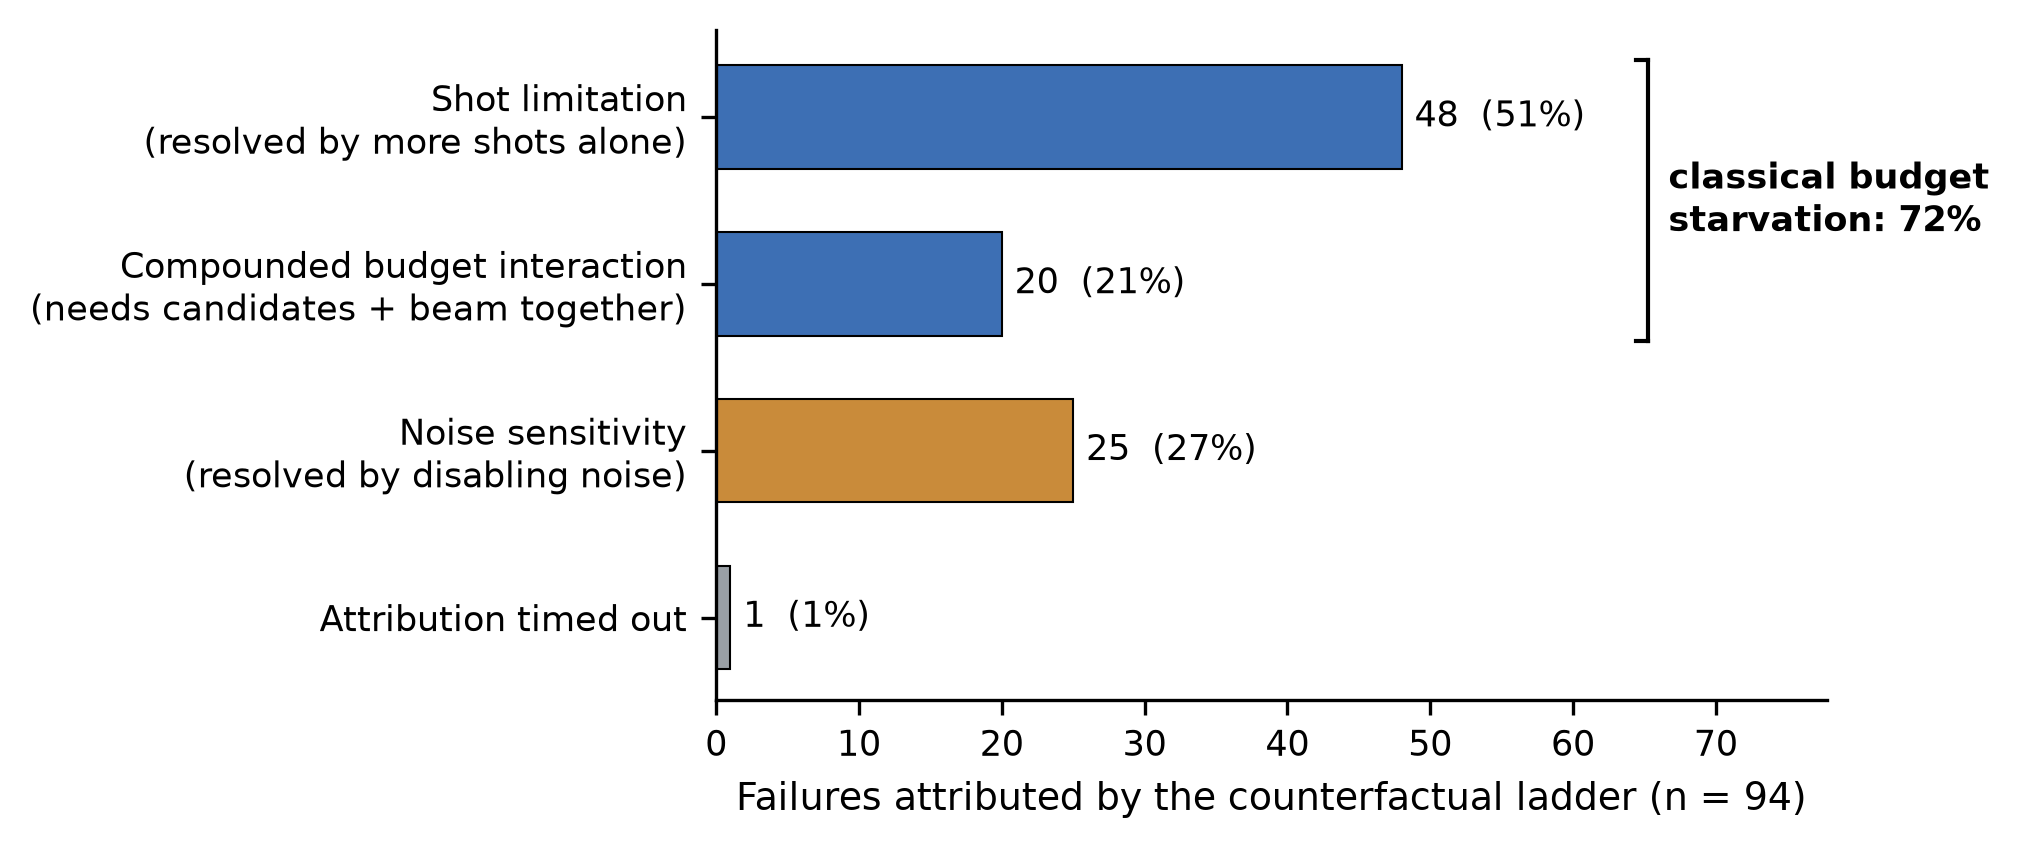
\includegraphics[width=\linewidth]{../Data/failure_study/plots/paper_fig2_failure_attribution.png}
\caption{\textbf{Which mechanism should a fix target?} Root-cause
attribution of all 94 failures observed anywhere in the characterisation
campaign, each replayed through the same counterfactual ladder and
assigned to the first rung that recovers it. Within this corpus the two
classical-budget mechanisms (blue) account for 72\% of failures between
them: 48 that
additional shots alone resolve, and 20 that resist every single-axis
relaxation and need candidate budget and beam width widened together.
Noise (orange) accounts for 27\%. This distribution is what selects the
classical reconstruction stage, rather than the circuit or the noise
model, as the place to intervene. Rendered from
\texttt{phase5\_attribution.csv}.}
\label{fig:pareto}
\end{figure}

% =====================================================================
